% SVN info for this file
\svnidlong
{$HeadURL$}
{$LastChangedDate$}
{$LastChangedRevision$}
{$LastChangedBy$}

\chapter{Topologia quoziente}
\labelChapter{topologia quoziente}

\begin{introduction}
‘‘La visione topologica del mondo, rilassata e flessibile, mi metteva a mio agio. La Geometria classica mi sembrava invece moralista e conservatrice. Se la Geometria si veste con un completo, la Topologia indossa maglietta e jeans.''
\begin{flushright}
	\textsc{David S. Richeson,} sarto topologico.
\end{flushright}
\end{introduction}
\lettrine[findent=1pt, nindent=0pt]{R}{iprendiamo} l'\textit{oggetto elasticamente magico} con cui abbiamo introdotto il \autoref{chap:spazitopologici}: fra tutte le deformazioni che potevamo fare, \textit{incollare} parti di esso \textit{non} era consentito. E se invece provassimo a farlo? Quello che otterremo non è più uno spazio ‘‘\textit{equivalente}'' per un topologo a quello originale, ma comunque con molte yrietà interessanti da studiare.\\
La \textbf{topologia quoziente} formalizza questo concetto euristico di ‘‘incollare parti'' utilizzando le \textit{relazioni di equivalenza}; con il tipico approccio della Topologia Generale, faremo ciò dando delle semplici (seppur inizialmente poco intuitive) condizioni sulla continuità in modo da definire la topologia più adatta per l'\textit{insieme quoziente}.
\section{Topologia quoziente}
Accenniamo fin da subito che la situazione è \textit{duale} rispetto a quella dei sottospazi, analizzati nella sezione \ref{sottospazi}, pag. \pageref{sottospazi}.
\begin{definition}{}[Topologia quoziente]
	Dato $X$ uno spazio topologico, $Y$ un \textit{insieme} e $\funct{}[f]{X}{Y}$ funzione suriettiva, la \textbf{topologia quoziente}\index{topologia!quoziente} su $Y$ indotta da $f$ è la topologia \textit{più fine} che rende $f$ continua.
\end{definition}
Dalla definizione si ha che $A\subseteq Y$ è un aperto della topologia quoziente se e solo se $f^{-1}(A)\subseteq X$ è aperto. Notiamo che l'implicazione $\rightimplies$ è necessaria affinché $f$ sia continua, mentre l'implicazione $\leftimplies$ è quella che caratterizza la topologia quoziente: infatti, se si considera un insieme $B\subseteq Y$ che non è aperto, allora la sua controimmagine $f^{-1}(B)\subseteq X$ non sarà aperta, altrimenti la topologia su $Y$ non sarebbe la più fine!
\begin{tipsandtricks}{n}
	Per verificare che un sottoinsieme sia aperto in $Y$ con la topologia quoziente bisogna verificare che la sua controimmagine è aperta.
\end{tipsandtricks}
Vediamo ora un esempio che giustifica la terminologia ‘‘topologia quoziente''.
\begin{example}{n}
	Sia $X$ uno spazio topologico e $\sim$ una relazione di equivalenza su $X$. Posto $Y=X/\!\sim$ l'insieme quoziente e
	\begin{equation*}
		\funct{}[\pi]{X}{Y}[x][\left[x\right]_\sim]
	\end{equation*}
	la \textbf{proiezione al quoziente}\index{proiezione!al quoziente}, la topologia quoziente su $Y$ è quella che rende la proiezione continua.
\end{example}
Ricordiamo il \textit{primo teorema fondamentale di isomorfismo} per gli \textit{insiemi}, altresì chiamato \textit{decomposizione canonica}.
\begin{remember}{n}[Primo teorema fondamentale di isomorfismo]~{}\\
	\begin{minipage}[t]{0.83\textwidth}
		Data una qualsiasi funzione suriettiva $\funct{}[f]{X}{Y}$ vi è la seguente relazione di equivalenza: 
		\begin{equation}
			\forall x,y\in X, \ x\sim y \iff f(x)=f(y)
		\end{equation}
		Inoltre, esiste ed unica $\funct{}[h]{X/\!\sim}{Y}$ biunivoca tale che $f=h\circ\pi$, ponendo $h\left( [x] \right) \coloneqq f(x)$ in modo tale che il diagramma \textit{commuti}.
	\end{minipage}
	\begin{minipage}[t]{0.13\textwidth}\vspace{-10pt}
		\begin{tikzcd}
			X \arrow[r, "f"] \arrow[d, "\pi"']                                   & Y \\
			X/\!\sim \arrow[ru, "\exists !h"', dotted] &
		\end{tikzcd}
	\end{minipage}
\end{remember}
\begin{proof}{n}
	Mostriamo che $h$ è ben definita e biunivoca. Poiché
	\begin{equation*}
		[x]=[y]\iff x\sim y\iff f(x)=f(y)\iff h([x])=h([y]),
	\end{equation*}
	si ha $h$ ben definita e iniettiva; la suriettività di $h$ segue da quella di $f$.\qedhere
\end{proof}

\subsection{Identificazione}
Tenendo a mente il concetto di \textit{immersione} illustrato a pagina \pageref{immersione}, definiamo il concetto duale di \textit{identificazione}.
\begin{definition}{}[Identificazione]
	Siano $X,Y$ spazi topologici e $\funct{}[f]{X}{Y}$ una funzione continua e suriettiva; $f$ si dice \textbf{identificazione}\index{identificazione} se $Y$ ha la topologia quoziente indotta da $f$.
\end{definition}
In generale è difficile determinare quando una data funzione è un'identificazione, quindi ne cerchiamo una condizione \textit{sufficiente}.
\begin{theorem}{}[Funzione continua, suriettiva, chiusa/aperta è identificazione chiusa/aperta; Manetti, 5.4]\label{condizione sufficiente identificazione}
Sia $\funct{}[f]{X}{Y}$ continua, suriettiva e chiusa (o aperta). Allora $f$ è un'identificazione chiusa (o aperta).
\end{theorem}
\begin{proof}{n}
	Supponiamo che $f$ sia aperta. Dimostrare che è un'identificazione è equivalente al mostrare che $A\subseteq Y$ aperto se e solo se $f^{-1}(A)\subseteq X$ aperto.\\
	$\rightimplies$ Segue dalla continuità di $f$.\\
	$\leftimplies$ Siccome $f$ è suriettiva allora vale $f(f^{-1}(A))=A$; essendo $f$ aperta segue che $A$ è aperto perché $f^{-1}(A)$ è aperto.\qedhere
\end{proof}
Vediamo ora un esempio di identificazione chiusa, ma \textit{non} aperta.
\begin{example}{n}
	Si consideri la funzione:
	\begin{equation*}
		\funct{}[f]{[0, \ 2\pi]}{S^1}[t][(\cos t, \ \sin t)].
	\end{equation*}
	È una funzione continua, suriettiva e chiusa essendo una funzione da un compatto a valori in uno spazio di Hausdorff, dunque è un'identificazione chiusa. Tuttavia, $f$ non è aperta: preso l'aperto $A=[0, \ 1)\subseteq [0, \ 2\pi]$, $f(A)$ non è aperto in $S^1$.
		\begin{center}
			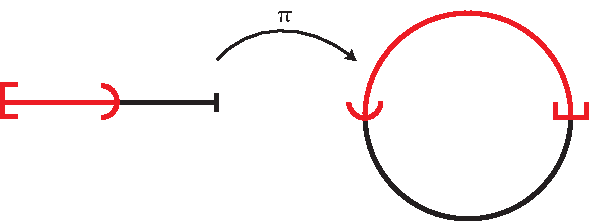
\includegraphics[trim=0cm 0cm 0cm 0cm,clip,scale=0.9]{images/half_circle-eps-converted-to.pdf}
		\end{center}
\end{example}
\begin{remark}{n}
	Gli \textit{omeomorfismi} sono identificazioni chiuse e aperte.
\end{remark}
Che relazione c'è fra identificazioni e quozienti dati da relazioni di equivalenza?
\begin{theorem}{n}[Proprietà universale delle identificazioni; Manetti, 5.6]~{}
\begin{minipage}[t]{0.83\textwidth}
	Dati $X,Y,Z$ spazi topologici, $g$ una qualsiasi funzione continua, $f$ identificazione con le mappe come in figura, allora esiste ed è unica $\funct{}[h]{Y}{Z}$ tale che $g=h\circ f$ se e solo se
		\begin{equation*}
			\forall x,y\in X, \ f(x)=f(y)\implies g(x)=g(y),
		\end{equation*}
		cioè se e solo se $g$ è costante sulle fibre di $f$.
\end{minipage}
	\begin{minipage}[t]{0.13\textwidth}\vspace{-10pt}
		\begin{tikzcd}
			X \arrow[r, "g"] \arrow[d, "f"'] & Z \arrow[from=2-1, to=1-2, "\exists ! h"', dotted] \\
			Y  &
		\end{tikzcd}
	\end{minipage}
\end{theorem}
\begin{proof}{n}
	Idealmente, se $f$ fosse invertibile definiremmo $h=g\circ f^{-1}$... tuttavia l'invertibilità di $f$ non è fra le ipotesi. Per ovviare a questo, utilizziamo la suriettività di $f$, considerando una controimmagine tramite $f$ e facendone l'immagine tramite $g$. Prendiamo dunque $y\in Y$ e poniamo
	\begin{equation*}
		h(y)\coloneqq g(x)\text{ per qualche }x\in f^{-1}(y).
	\end{equation*}
	Questa costruzione $h$ è ben definita siccome $g$ è costante sulle fibre di $f$. Verifichiamo che $h$ è continua tramite la definizione:
		\begin{gather*}
			U\subseteq Z \text{ aperto }, \ h^{-1}(U)\subseteq Y \iff f^{-1}(h^{-1}(U))\subseteq X \text{ aperto} \iff g^{-1}(U)\subseteq X \text{ aperto}
		\end{gather*}
	Siccome $g$ è continua, allora lo è anche $h$.\qedhere
\end{proof}
\begin{minipage}[t]{0.83\textwidth} \label{proprietà identificazione quoziente e mappa continua indotta}
Data allora $f$ continua, $\sim$ relazione di equivalenza e $X/\!\sim$ spazio topologico con la topologia quoziente indotta dalla proiezione $\pi$, esiste $\funct{}[g]{X/\!\sim}{Y}$ continua se e solo se
\begin{equation*}
	x\sim y \implies f(x)=f(y),
\end{equation*}
ossia se e solo se $f$ è costante sulle fibre di $\pi$.
\end{minipage}
\begin{minipage}[t]{0.16\textwidth}\vspace{-10pt}
 		\begin{tikzcd}
		 	X \arrow[r, "f"] \arrow[d, "\pi"']                                   & Y \\
 			X/\!\sim \arrow[ur, "g"', dotted] &
		\end{tikzcd}
	\end{minipage}\\
\hspace{-1mm}
\begin{minipage}[t]{0.83\textwidth}\vspace{2mm}
In particolare, se $\sim$ è la relazione d'equivalenza indotta da $f$, e dunque si è nelle ipotesi del \textit{primo teorema fondamentale di isomorfismo} degli \textit{insiemi}, allora
\begin{equation*}
	x\sim y \iff f(x)=f(y)
\end{equation*}
induce l'esistenza di un'unica funzione $\overline{f}$ \textit{biettiva} e \textit{continua} tale che $f=\overline{f}\circ \pi$. Dunque vale:
	 	\end{minipage}
	\begin{minipage}[t]{0.16\textwidth}\vspace{-1pt}
			\begin{tikzcd}
				X \arrow[r, "f"] \arrow[d, "\pi"']                                   & Y \\
				X/\!\sim \arrow[ur, "\overline{f}"', dotted] &
			\end{tikzcd}
	\end{minipage}\vspace{-1.5mm}\\
\begin{equation*}
	\overline{f} \text{ omeomorfismo} \iff f \text{ identificazione}
\end{equation*}
\vspace{-1.5mm}\noindent Riprendiamo l'esempio precedente ed esaminiamolo in termini di spazio quoziente.
\begin{example}{}[{$D^n/\!\sim\cong S^n$}]
	Consideriamo il caso $n=1$:
	\begin{equation*}
		\funct{}[f]{D^1=[0, \ 2\pi]}{S^1}[t][(\cos t, \ \sin t)].
	\end{equation*}
	La funzione $f$ è un identificazione in quanto continua, suriettiva e chiusa perché funzione da un compatto a valori in un Hausdorff; pertanto
	\begin{equation*}
		S^1\cong [0, \ 2\pi]/\!\sim\cong \unint/\!\sim=D^1/\!\sim, 
	\end{equation*}
	con $\sim$ la relazione indotta da $f$:
	\begin{equation*}
		 s\sim t \iff \begin{cases}
			\cos s=\cos t \\
			\sin s =\sin t
		\end{cases} \iff s=t  \vee s=0,\ t=2\pi.
	\end{equation*}
	Si può generalizzare in dimensione $n$ con l'identificazione
	\begin{equation*}
		\funct{}[f]{D^n}{S^n}[\mathbf{x}][\left( 2\mathbf{x}\sqrt{1- \| \mathbf{x} \|^2}, \ 2\| \mathbf{x}\|^2 -1 \right)].
	\end{equation*}
	Dunque $D^n/\!\sim\cong S^n$ per la relazione
\begin{equation*}
	\mathbf{x}\sim \mathbf{y} \iff \mathbf{x}=\mathbf{y} \vee \norm{\mathbf{x}}  ^2 = 1 = \| \mathbf{y} \|^2.
\end{equation*}
	In altre parole, ogni punto interno è \textit{in relazione con sé stesso} e tutti i punti sul bordo sono \textit{identificati} in un unica classe.
\end{example}
% LEZ 12
\subsection{Quozienti tipici}
Vedremo ora degli esempi di spazi quoziente usati frequentemente.
\begin{intuitively}{n}
	Quando quozientiamo uno spazio topologico, possiamo immaginare che i punti contenuti nelle classi di equivalenza vengano ‘‘\textit{incollati}'' tutti in un unico punto per formare un nuovo spazio quoziente. Ad esempio, prendendo il disco $D^2$ con la relazione di equivalenza $\sim$ che identifica i punti del bordo:
	\begin{equation*}
		(x_1,\ y_1) \sim (x_2,\ y_2)\iff (x_1,\ y_1)=(x_2,\ y_2) \text{ oppure } x_1^2 +y_1^2= x_2^2 +y_2^2=1
	\end{equation*}
	I punti all'\textit{interno del disco} vengono tutti identificati in classi di equivalenza \textit{separate}, dunque passando allo spazio quoziente avremo una classe per \textit{ciascun} punto interno e un'\textit{unica} classe per tutti il bordo. Lo spazio quoziente ottenuto è $S^2$: possiamo ottenerlo visualmente ‘‘gonfiando'' l'interno del disco per poi chiudere il ‘‘palloncino'' ottenuto lungo i punti del bordo, come nella figura seguente.
	\begin{center}
		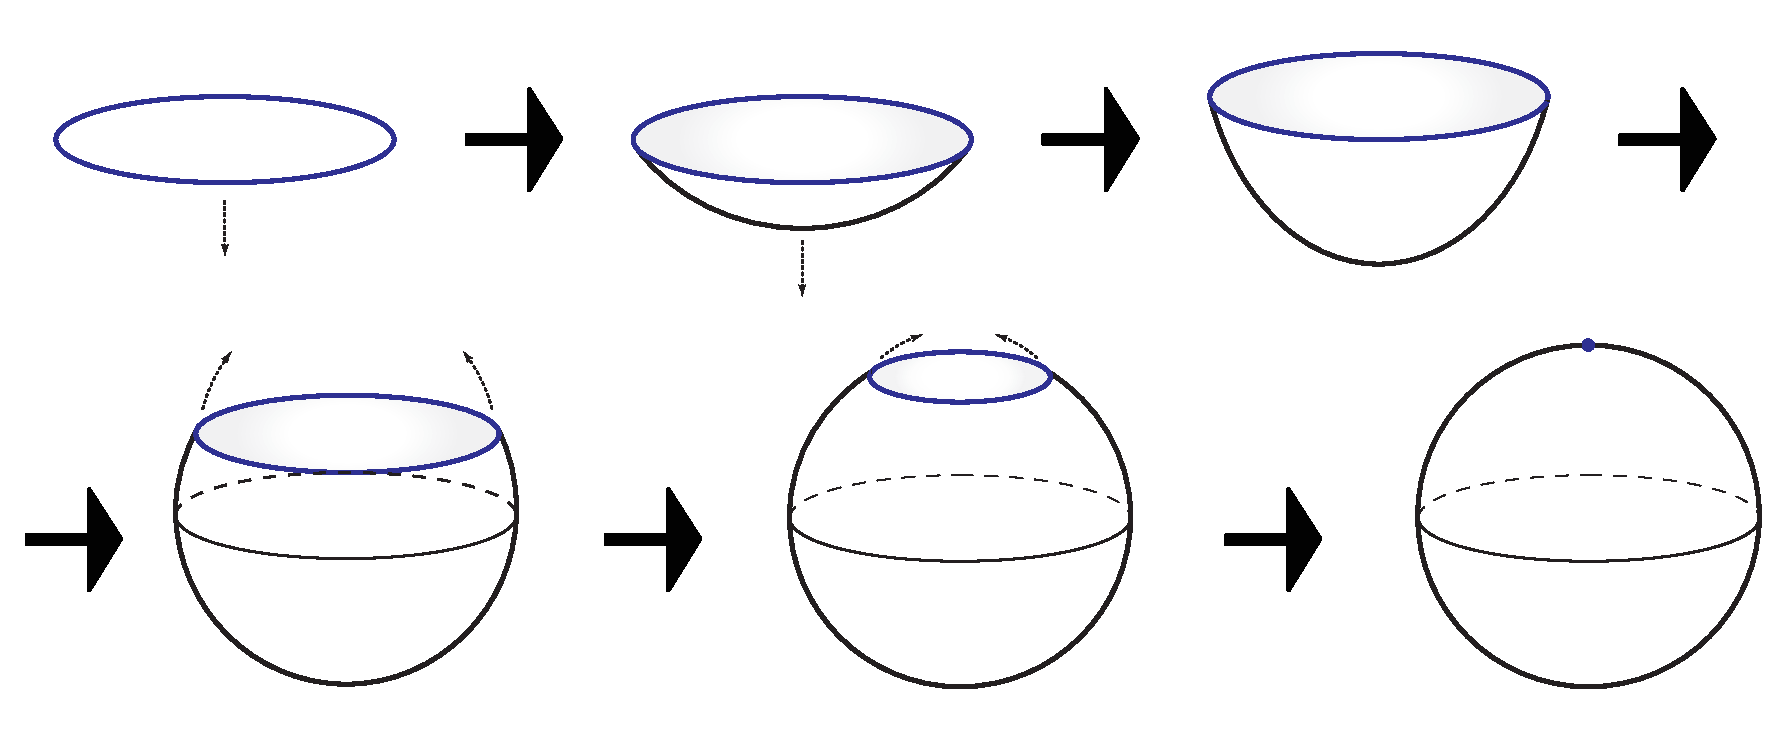
\includegraphics[trim=0cm 0cm 0cm 0cm,clip,scale=0.4]{images/disctosphere.pdf}
	\end{center}
\end{intuitively}
\subsubsection{Contrazione di un sottospazio ad un punto}
Sia $X$ uno spazio topologico, $A\subseteq X$. Su $X$ consideriamo la relazione d'equivalenza
\begin{equation*}
	x\sim y\iff x=y\ \text{oppure}\ x,y\in A,
\end{equation*}
ovvero ogni punto è in relazione con sé stesso e tutti i punti di $A$ sono in relazione fra loro, dunque quozientando si ‘‘\textbf{contraggono}''\index{contrazione} ad un unico punto.
\begin{example}{}[{$D^n/S^{n-1}\cong S^n$}]
Cerchiamo ora di generalizzare l'esempio precedente. Ricordiamo che relazione c'è fra i dischi e le sfere:
		\begin{gather*}
			D^n=\text{ disco in } \R^n=\{\mathbf{x}\in\R^n \mid \norm{\mathbf{x}} \leq 1 \}\\
			S^{n-1}=\text{ bordo di } D^n=\{\mathbf{x}\in\R^n \mid \norm{\mathbf{x}} = 1 \}.
		\end{gather*}
	Considerando $\sim$ come la contrazione di $S^{n-1}$ ad un punto, si ha che $D^n/S^{n-1} \cong S^n$.
\end{example}

\begin{warning}{n}
	Anche se $X$ è di Hausdorff non è detto che $X/A$ sia di Hausdorff!	Se $A$ non è chiuso allora $X/A$ non è neanche T1: infatti, $\pi^{-1}([A])=A$ \textit{non} chiuso implica che $[A]$ \textit{non} lo è, quindi per la caratterizzazione degli spazi T1 (definizione \ref{T1}, pag. \pageref{T1}) $X/A$ non è T1. Tuttavia, se $X$ è di Hausdorff, $K\subseteq X$ è compatto allora $X/K$ è di Hausdorff. Nelle ‘‘Note aggiuntive'', a pag. \pageref{quozientehausdorffsuspaziocompatto}, si può trovare la dimostrazione di ciò.
\end{warning}
\subsubsection{Cono su uno spazio}
\begin{definition}{}[Cilindro]
	Dato $X$ spazio topologico, si definisce \textbf{cilindro}\index{cilindro} su $X$ lo spazio $X\times \unint$.
\end{definition}
\begin{definition}{}[Cono]
	Il \textbf{cono}\index{cono} su $X$ spazio topologico è il quoziente
	\begin{equation*}
		 C\left(X\right)=\left(X\times\unint\right)/\left(X\times\{1\}\right)\ \text{oppure}\ C\left(X\right)=\left(X\times\unint\right)/\left(X\times\{0\}\right).
	\end{equation*}
\end{definition}
\begin{intuitively}{n}
	Riprendiamo il procedimento intuitivo di incollare parti dello spazio originale per creare il quoziente per creare il \textit{cono} dal \textit{cilindro}: in questo caso, tutti i punti di una delle basi vengono incollati in uno.
\begin{center}
	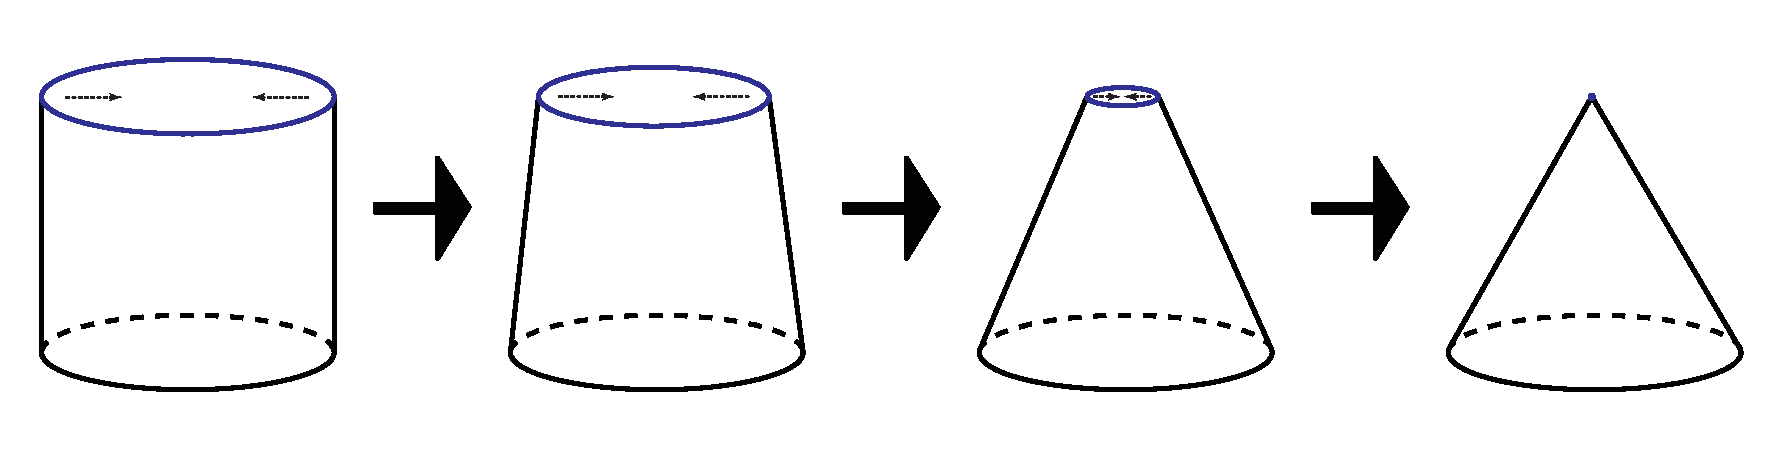
\includegraphics[trim=0cm 0cm 0cm 0cm,clip,scale=0.4]{images/cilindertocone.pdf}
\end{center}
\end{intuitively}
\begin{remark}{n}
	Un cono è sempre c.p.a. rispetto al ‘‘vertice''.
\end{remark}
\begin{example}{}[\textsc{Cono su} ${S^n \cong D^{n+1}}$]
	Studiamo i casi al variare della dimensione.\\
	$\underbfsf{n=0:}$ $S^0=\{-1, \ 1\}=X \rightsquigarrow X\times\unint \rightsquigarrow \left(X\times\unint\right)/\left(X\times \{0\}\right) \cong D^1$.
\begin{center}
	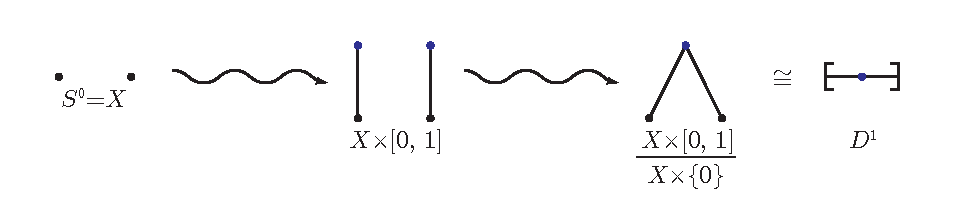
\includegraphics[trim=0cm 0cm 0cm 0cm,clip,scale=0.9]{images/cones0.pdf}
\end{center}
	$\underbfsf{n=1:}$ $S^1=X \rightsquigarrow X\times\unint \rightsquigarrow \left(X\times\unint\right)/\left(X\times \{0\}\right) \cong D^2$.
\begin{center}
	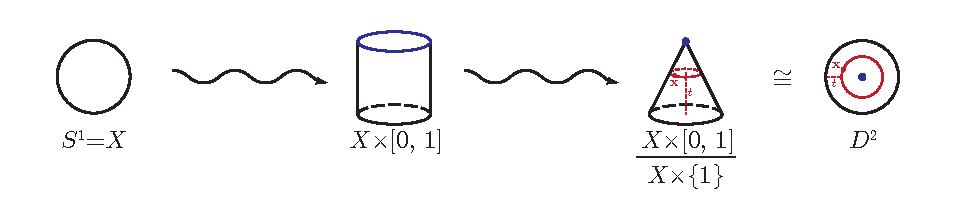
\includegraphics[trim=0cm 0cm 0cm 0cm,clip,scale=0.9]{images/cones1.pdf}
\end{center}
	In generale, considerata la funzione
	\begin{equation*}
		\funct{}[f]{S^n\times\unint}{D^{n+1}}[(\mathbf{x}, \ t)][t\mathbf{x}],
	\end{equation*}
\begin{minipage}[t]{0.72\textwidth}
	essa è continua, suriettiva, chiusa perché funzione da un compatto a valori in un Hausdorff, dunque $f$ è identificazione e induce l'omeomorfismo $\overline{f}$ tra il cono $C\left(S^n\right)$ e il disco $D^{n+1}$. Verifichiamo che la relazione di equivalenza indotta da $f$ è proprio quella di contrazione:
\end{minipage}
\begin{minipage}[t]{0.29\textwidth}\vspace{-10pt}
	\begin{tikzcd}
		{S^{n}\times\unint} & {D^{n+1}} \\
		{C\left(X\right)}
		\arrow["f", from=1-1, to=1-2]
		\arrow["\pi"', from=1-1, to=2-1]
		\arrow["{\overline{f}}"', from=2-1, to=1-2]
	\end{tikzcd}
\end{minipage}
\begin{equation*}
	(\mathbf{x}, \ t)\sim (\mathbf{y}, \ s) \iff f(\mathbf{x}, \ t)=f(\mathbf{y}, \ s) \iff t\mathbf{x}=s\mathbf{y} \iff \begin{cases}
		\mathbf{x=y}, \ t=s \\
		t=s=0
	\end{cases}
\end{equation*}
Se $t\neq 0$, $\mathbf{x}=\frac{s}{t}\mathbf{y}$, ma allora
	\begin{equation*}
		\norm{\mathbf{x}}=1  \implies \left| \frac{s}{t} \right| \underbrace{\norm{\mathbf{y}}}_{=1}=1 \implies \left| \frac{s}{t} \right| =1 \implies s=t \implies \mathbf{x=y}
	\end{equation*}
\end{example}
\subsubsection{Retta con due origini} \label{retta 2 origini}
Analizziamo un particolare spazio topologico che spesso funge da controesempio (ad esempio per le varietà topologiche, sez. \ref{retta2originivarietà}, pag. \pageref{retta2originivarietà}): \textbf{la retta con due origini}. Sia $X=\R\times\{a,b\}$.
\begin{center}
	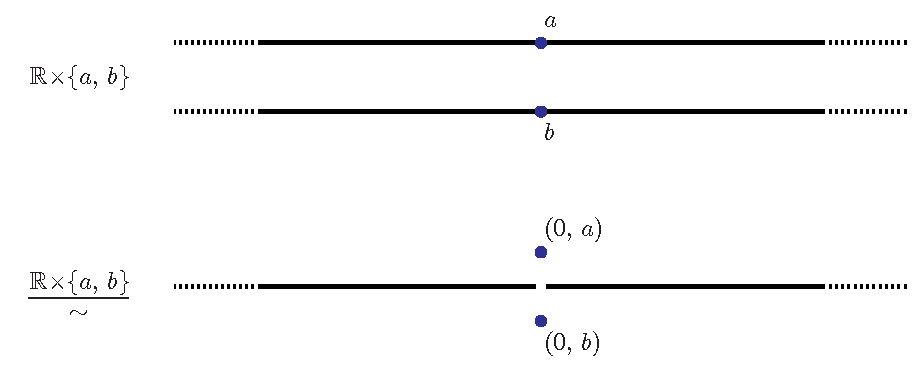
\includegraphics[trim=0cm 0cm 0cm 0cm,clip,scale=0.95]{images/line2origins.pdf}
\end{center}
Vogliamo definire una relazione di equivalenza che lasci ‘‘separate'' solo le origini:
	\begin{gather*}
		(x, \ \alpha)\sim (y, \ \beta) \iff
			\begin{cases}
				x=y,\ \alpha=\beta \\
				x=y\neq 0
			\end{cases}		
	\end{gather*}
\begin{property}{n}[Retta con due origini]
	\begin{enumerate}
		\item $Y\coloneqq X/\!\sim$ è c.p.a..
		\item $Y$ non è di Hausdorff.
		\item $Y$ è \textit{localmente omeomorfo} a $\R$.
		\item Esistono $K_1, \ K_2\subseteq Y$ compatti tali per cui $K_1\cap K_2$ \textit{non} è compatto.
	\end{enumerate}
\end{property}
\begin{proof}{n}~{}
		\begin{enumerate}[label=\Roman*]
		\item Se i punti $[(x, \ \alpha)]$ e $[(y, \ \beta)]$ sono tali che $x\neq 0 \neq y$, basta prendere il segmento $\overline{xy}$ sulla retta $\R\times\{a\}$ e proiettarlo. Per unire $[(0,\ a)]$ e $[(0, \ b)]$ basta unire entrambi con un cammino al punto $[(1, \ a)]=[(1, \ b)]$.
		\item Tutti gli intorni di $[(0, \ a)]$ si intersecano con tutti gli intorni di $[(0, \ b)]$.
		\item Ogni punto ha un intorno omeomorfo ad un intervallo aperto di $\R$.
		\item Basta prendere $K_1=\pi\left([-1, \ 1]\times \{a\} \right)$ e $K_2=\pi\left([-1, \ 1]\times \{b\} \right)$ compatti in $Y$, ma $K_2\cap K_2= [-1,\ 0) \cup (0,\ 1]$ \textit{non} è compatto in $Y$.\qedhere
	\end{enumerate}
\end{proof}
\subsection{Quoziente di Hausdorff}
Cerchiamo ora delle condizioni per avere un \textit{quoziente di} Hausdorff.
\begin{theorem}{}[Condizioni sufficienti per il quoziente di Hausdorff]\label{quozientehausdorff}
Sia $\funct{}[f]{X}{Y}$ continua e identificazione con $X$ compatto e di Hausdorff. Sono equivalenti:
		\begin{enumerate}
			\item $Y$ è di Hausdorff.
			\item $f$ chiusa.
			\item $K=\Set{ (x_1,\ x_2)\in X\times X | f(x_1)=f(x_2)}$ chiuso in $X\times X$.
		\end{enumerate}
\end{theorem}
\begin{proof}{n}~{}\\
	$1 \implies 3)$  Poichè $Y$ è di Hausdorff, la diagonale $\Delta_Y$ è chiusa (teorema \ref{hausdorff diagonale chiusa}, pag. \pageref{hausdorff diagonale chiusa}). Si consideri ora la seguente funzione:
	\begin{equation*}
		\funct{}[h\coloneqq f\times f]{X\times X}{Y\times Y}[(x_1,\ x_2)][\left( f(x_1), \ f(x_2) \right)]
	\end{equation*}
	Essa è continua perché lo è $f$. Notiamo che $K=h^{-1}(\Delta_Y)$: allora $K$ è chiuso in quanto controimmagine della diagonale, chiusa per ipotesi di Hausdorff.
	\[\begin{tikzcd}
		X &&&& Y \\
		& {X\times X} && {Y\times Y} \\
		X &&&& Y
		\arrow["{h\coloneqq f\times f}", from=2-2, to=2-4]
		\arrow["{p_1}"', two heads, from=2-2, to=1-1]
		\arrow["{p_2}", two heads, from=2-2, to=3-1]
		\arrow["{q_2}"', two heads, from=2-4, to=3-5]
		\arrow["{q_1}", two heads, from=2-4, to=1-5]
		\arrow["f"', from=3-1, to=3-5]
		\arrow["f", from=1-1, to=1-5]
	\end{tikzcd}\]
	$3\implies 2)$ Per dimostrare che $f$ è chiusa bisogna far vedere che per ogni $C\subseteq X$ chiuso $f(C)\subseteq Y$ è chiuso; $Y$ ha la topologia quoziente perché $f$ è identificazione, quindi dobbiamo mostrare che $f^{-1}\left(f(C)\right)\subseteq X$ sia chiuso. Notiamo che $f^{-1}\left(f(C)\right)= p_1(K\cap p_2^{-1}(C))$; noto che $p_2^{-1}(C)=X\times C$ si ha che
	\begin{align*}
		K\cap p_2^{-1}(C) & = \left\{ (x_1,\ x_2)\in X\times X \mid f(x_1)=f(x_2)\in f\left(C\right) \right\}\\
		& = \left\{ (x_1,\ x_2)\in X\times X \mid x_1\in f^{-1}\left(f\left(C\right)\right) \right\},
	\end{align*}
	da cui
	\begin{equation*}
		p_1(K\cap p_2^{-1}(C)) = \Set{(x_1,\ x_2)\in X\times X | x_1\in f^{-1}\left(f\left(C\right)\right)}=f^{-1}\left(f(C)\right).
	\end{equation*}
	Concludiamo che $f$ è chiusa in base alle proprietà delle proiezioni $p_1$ e $p_2$:
	\begin{itemize}
		\item poiché $p_2$ continua e $C$ chiuso, $p_2^{-1}(C)$ è chiuso;
		\item poiché $K$ chiuso, $p_2^{-1}(C)\cap K$ è chiuso;
		\item poiché $X$ compatto implica che $p_1$ chiusa, si ha che $p_1(K\cap p_2^{-1}(C))=f^{-1}\left(f(C)\right)$ è chiuso.
	\end{itemize}
	$2\implies 1)$ Serve il \textit{teorema di Wallace}, pertanto non ne affronteremo la dimostrazione.
\end{proof}
\begin{remark}{n}
	Nella dimostrazione $1\implies 3)$ \textit{non} si è utilizzato che $f$ è un'identificazione, dunque vale \textit{in generale}!
\end{remark}
